\section{From a regular expression to a finite state automaton}

Several algorithms can transform a regular expression into an automaton, differing in their characteristics. 
The three main methods are:
\begin{enumerate}
    \item \textit{Thompson (structural) method}.
    \item \textit{Glushkov McNaughton Yamada method}.
    \item \textit{Berry-Sethi method}.
\end{enumerate}

\subsection{Locally testable language}
\begin{definition}[\textit{Initials set}]
    The set of initials is defined as: 
    \[\textnormal{Ini}(L)=\{a \in \Sigma \mid  a\Sigma^{\ast}\cap L \neq \varnothing\}\]
\end{definition}
To compute the sets of initials we use the following rules: 
\begin{itemize}
    \item $\textnormal{Ini}(\varnothing)=\varnothing$.
    \item $\textnormal{Ini}(\varepsilon)=\varnothing$.
    \item $\textnormal{Ini}(a)=\{a\} \textnormal{ for every character }a$.
    \item $\textnormal{Ini}(e \cup e^{\prime})=\textnormal{Ini}(e) \cup \textnormal{Ini}(e^{\prime})$.
    \item $\textnormal{Ini}(e \cdot e^{\prime})=\textnormal{if Null}(e) \textnormal{ then Ini}(e)\cup\textnormal{Ini}(e^{\prime}) \textnormal{ else Ini}(e)$.
    \item $\textnormal{Ini}(e^{\ast})=\textnormal{Ini}(e^{+})=\textnormal{Ini}(e)$.
\end{itemize}
\begin{definition}[\textit{Finals set}]
    The set of finals is defined as: 
    \[\textnormal{Fin}(L)=\{a \in \Sigma \mid  \Sigma^{\ast}a\cap L \neq \varnothing\}\]
\end{definition}
To compute the sets of finals we use the following rules: 
\begin{itemize}
    \item $\textnormal{Fin}(\varnothing)=\varnothing$.                                                                                                         
    \item $\textnormal{Fin}(\varepsilon)=\varnothing$.                                                                                                         
    \item $\textnormal{Fin}(a)=\{a\} \textnormal{ for every character }a$.                                                                                     
    \item $\textnormal{Fin}(e \cup e^{\prime})=\textnormal{Fin}(e) \cup \textnormal{Fin}(e^{\prime})$.                                                                   
    \item $\textnormal{Fin}(e \cdot e^{\prime})=\textnormal{if Null}(e^{\prime}) \textnormal{ then Fin}(e)\cup\textnormal{Fin}(e^{\prime}) \textnormal{ else Fin}(e^{\prime})$.    
    \item $\textnormal{Fin}(e^{\ast})=\textnormal{Fin}(e^{+})=\textnormal{Fin}(e)$.                                                                               
\end{itemize}
\begin{definition}[\textit{Digrams set}]
    The set of digrams is defined as: 
    \[\textnormal{Dig}(L)=\{x \in \Sigma^{2} \mid  \Sigma^{\ast}x\Sigma^{\ast} \cap L \neq \varnothing\}\]
\end{definition}
To compute the sets of digrams we use the following rules: 
\begin{itemize}
    \item $\textnormal{Dig}(\varnothing)=\varnothing$.                                                                                                     
    \item $\textnormal{Dig}(\varepsilon)=\varnothing$.                                                                                                       
    \item $\textnormal{Dig}(a)=\varnothing \textnormal{ for every character }a$.                                                                                   
    \item $\textnormal{Dig}(e \cup e^{\prime})=\textnormal{Dig}(e) \cup \textnormal{Dig}(e^{\prime})$.                                                                 
    \item $\textnormal{Dig}(e \cdot e^{\prime})=\textnormal{Dig}(e) \cup \textnormal{Dig}(e^{\prime}) \cup \textnormal{Fin}(e) \cdot \textnormal{Ini}(e^{\prime})$.    
    \item $\textnormal{Dig}(e^{\ast})=\textnormal{Dig}(e^{+})=\textnormal{Dig}(e) \cup \textnormal{Fin}(e) \cdot \textnormal{Ini}(e)$.                                                                 
\end{itemize}
\begin{definition}[\textit{Forbidden digrams set}]
    The set of forbidden digrams is defined as: 
    \[\overline{\textnormal{Dig}(L)}=\Sigma^{2} \setminus\textnormal{Dig}(L)\]
\end{definition}
\begin{definition}[\textit{Locally testable language}]
    The language $L$ is called locally testable, if and only if it satisfies the following identity: 
    \[L\setminus\{\varepsilon\}=\{x\mid \textnormal{Ini}(x)\in \textnormal{Ini}(L) \land \textnormal{Fin}(x)\in \textnormal{Fin}(L)\land \textnormal{Dig}(x)\subseteq \textnormal{Dig}(L)\}\]
\end{definition}
\begin{example}
    Consider the language $L_1=(abc)^{\ast}$. 
    The sets defined for $L_1$ in this case are:
    \begin{itemize}
        \item $\textnormal{Ini}(L_1)=\{a\}$.
        \item $\textnormal{Fin}(L_1)=\{c\}$.
        \item $\textnormal{Dig}(L_1)=\{ab,bc,ca\}$.
        \item $\overline{\textnormal{Dig}(L)}=\{aa,ac,ba,bb,cb,cc\}$
    \end{itemize}
\end{example}

\paragraph*{Local language recognizer}
To create a recognizer for a local language, we examine the input string sequentially from left to right, verifying the following conditions: the starting character belongs to the Ini set, every digram is a member of Dig, and the concluding character is part of the Fin set. 
The acceptance of the string hinges on the success of all these checks.
This recognition process can be implemented using a sliding window approach with a width of two characters, sliding over the input string from left to right. 
At each step of the sliding window, the contents are inspected. 
If the window reaches the end of the string and all checks succeed, the string is accepted; otherwise, it is rejected. 
This sliding window algorithm lends itself to straightforward implementation through a nondeterministic automaton.
The recognizer associated with the sets Ini, Fin, and Dig possesses the following characteristics:
\begin{itemize}
    \item \textit{Initial states}: $q_0 \cup \Sigma$.
    \item \textit{Final states}: Fin.
    \item \textit{Transitions}: $q_0 \overset{a}{\rightarrow}a$ if $a \in$ Ini, and $b \overset{a}{\rightarrow}b$ if $ab \in$ Dig.
\end{itemize}
If the language includes the empty string, the initial state $q_0$ is also designated as final.
\begin{example}
    The automaton designed to recognize the language $L_1=(abc)^{\ast}$ is depicted below: 
    \begin{figure}[H]
        \centering
        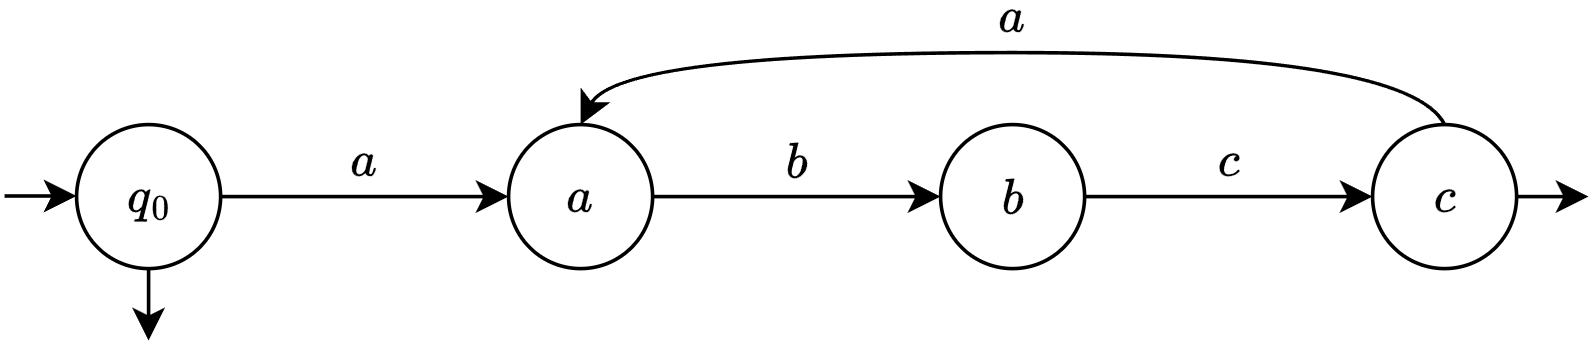
\includegraphics[width=0.75\linewidth]{images/local.png}
    \end{figure}
\end{example}
\begin{definition}[\textit{Linear regular expression}]
    A regular expression is termed linear if it does not contain any repeated generators.
\end{definition}
\begin{property}
    The languages generated by linear regular expressions are local. 
\end{property}
Linearity ensures that the subexpressions of a regular expression are defined over distinct alphabets. 
Since a regular expression is the composition of its subexpressions, the language generated by a linear regular expression becomes local due to the closures of local languages over disjoint alphabets. 
It's important to note that the converse does not hold.
This observation implies that constructing a recognizer for a general regular language simplifies to determining the characteristic local sets (Ini, Fin, Dig) for such a language, provided the alphabet undergoes slight modification.

\paragraph*{Empty string generation}
To verify whether a regular expression $e$ generates the empty string, the Null$(e)$ operator can be employed. 
This operator evaluates to true when the empty string is part of the regular expression and false otherwise. 
The functioning of Null$(e)$ is outlined as follows:
\begin{itemize}
    \item $\textnormal{Null}(\varnothing)=\textnormal{false}$. 
    \item $\textnormal{Null}(\varepsilon)=\textnormal{true}$. 
    \item $\textnormal{Null}(a)=\textnormal{false for every character } a$.
    \item $\textnormal{Null}(e \cup e^{\prime})=\textnormal{Null}(e) \lor \textnormal{Null}(e^{\prime})$.
    \item $\textnormal{Null}(e \cdot e^{\prime})=\textnormal{Null}(e) \land \textnormal{Null}(e^{\prime})$.
    \item $\textnormal{Null}(e^{\ast})=\textnormal{true}$. 
    \item $\textnormal{Null}(e^{+})=\textnormal{Null}(e)$. 
\end{itemize}

\subsection{Thompson structural method}
The Thompson structural method modifies the original automaton to have unique initial and final states.
It is is based on the correspondence of regular expression and recognizer automaton. 
The rules used to find the automaton are the following: 
\begin{figure}[H] 
    \begin{minipage}[b]{0.5\linewidth}
        \centering
        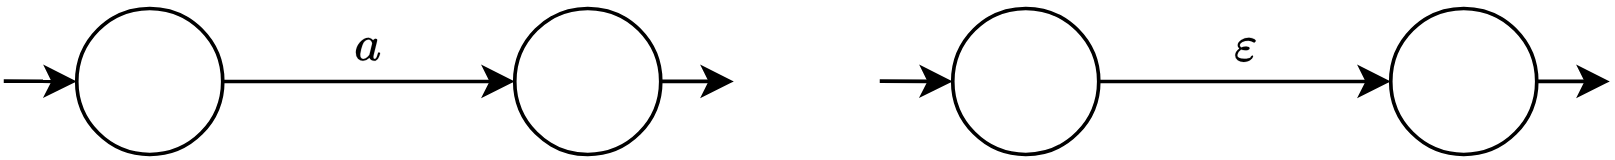
\includegraphics[width=.9\linewidth]{images/t1.png} 
        \caption*{Atomic expressions} 
        \vspace{4ex}
    \end{minipage}%%
    \begin{minipage}[b]{0.5\linewidth}
        \centering
        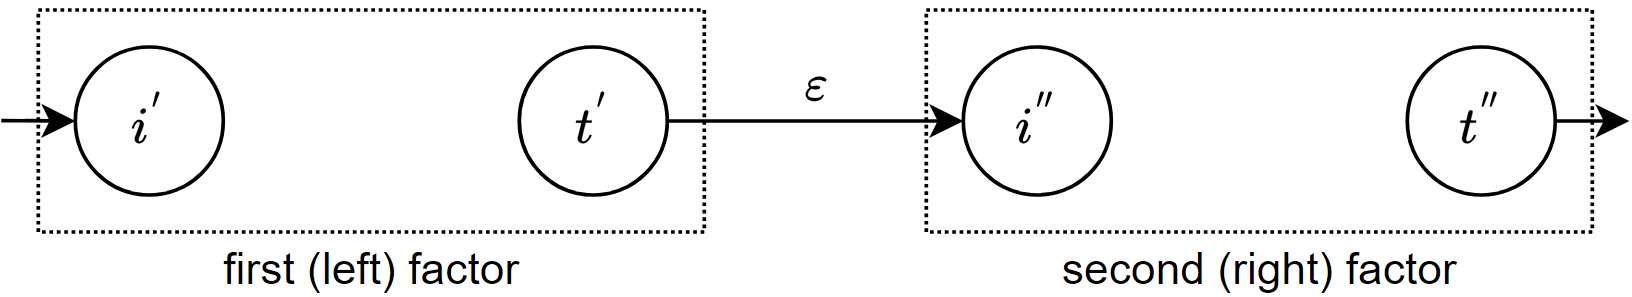
\includegraphics[width=.9\linewidth]{images/t2.png} 
        \caption*{Concatenation} 
        \vspace{4ex}
    \end{minipage} 
    \begin{minipage}[b]{0.5\linewidth}
        \centering
        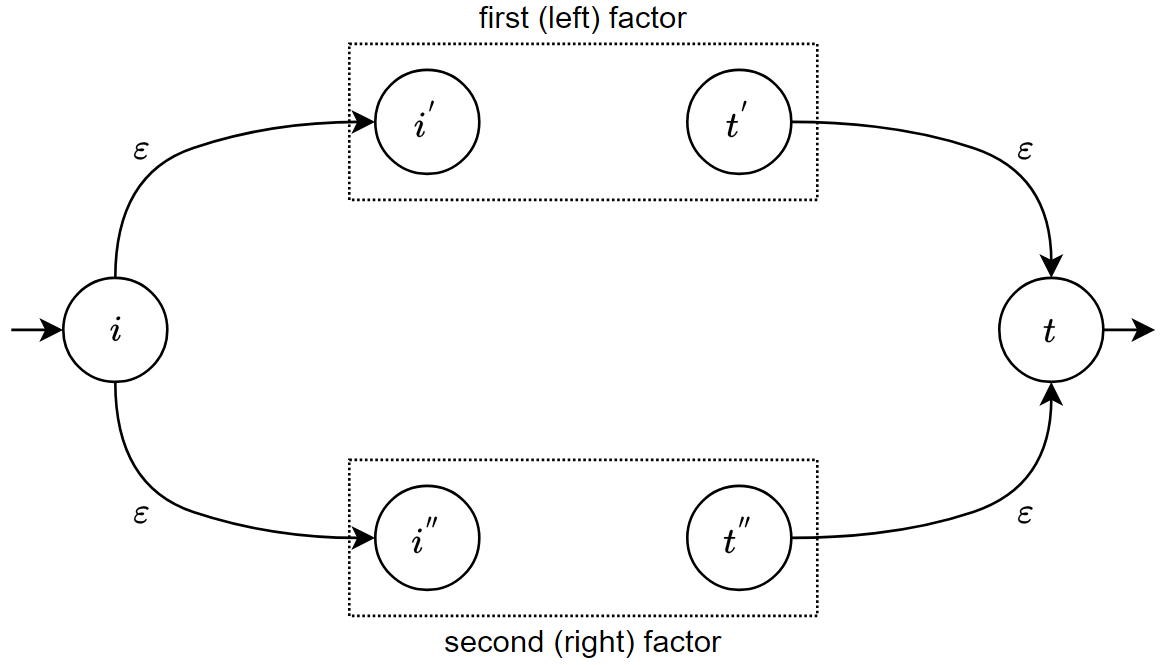
\includegraphics[width=.8\linewidth]{images/t3.png} 
        \caption*{Union} 
        \vspace{4ex}
    \end{minipage}%% 
    \begin{minipage}[b]{0.5\linewidth}
        \centering
        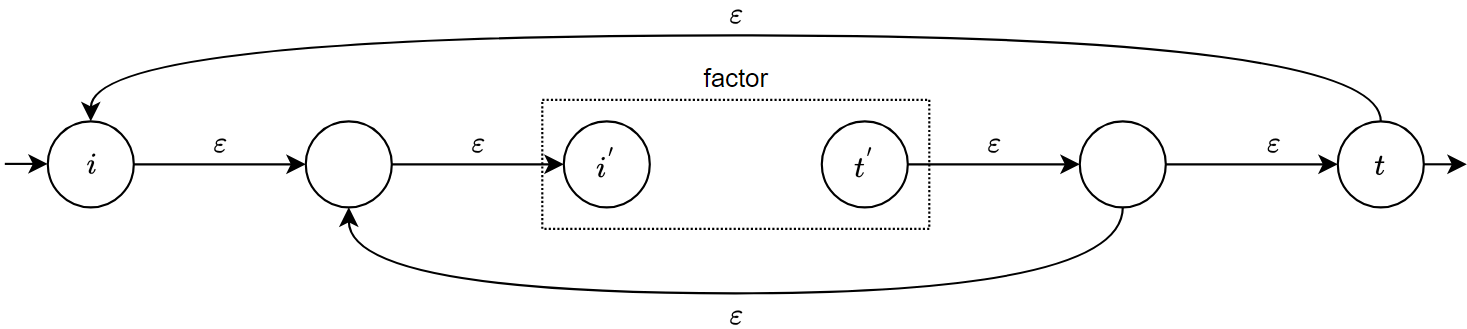
\includegraphics[width=.9\linewidth]{images/t4.png} 
        \caption*{Star closure} 
        \vspace{4ex}
    \end{minipage} 
\end{figure}
In general, the outcome of the Thompson method is a nondeterministic automaton with spontaneous moves. 
This method is an application of the closure properties of regular languages under the operations of union, concatenation, and star.
\begin{example}
    Consider the regular expression $(a \cup \varepsilon)b^{\ast}$. 
    Rewriting the same regular expression with symbols and subexpression indexing yields:
    \[\left(_1\left(_2\left(_3a\right)_4 \cup \left(_5\varepsilon\right)_6\right)_7\left(_8\left(_9b\right)_{10}\right)_{11}^{\ast}\right)_{12}\]
    The corresponding structure tree is as follows:
    \begin{figure}[H]
        \centering
        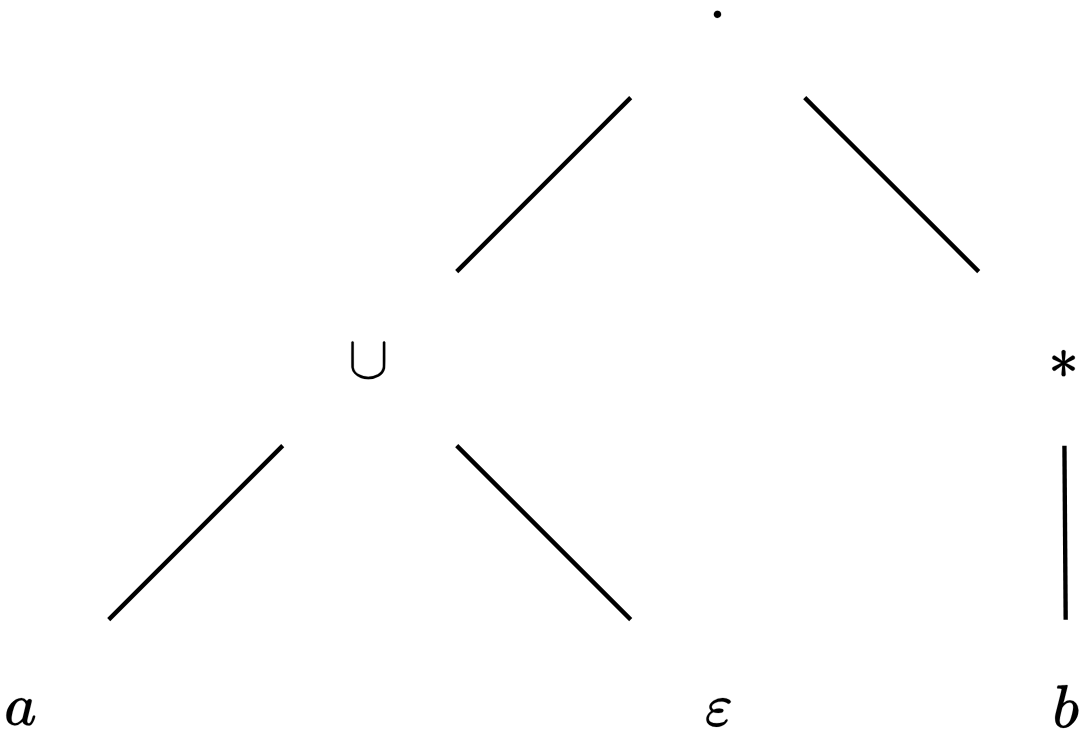
\includegraphics[width=0.35\linewidth]{images/st.png}
    \end{figure}
    By applying the rules from the table, the resulting automaton is:
    \begin{figure}[H]
        \centering
        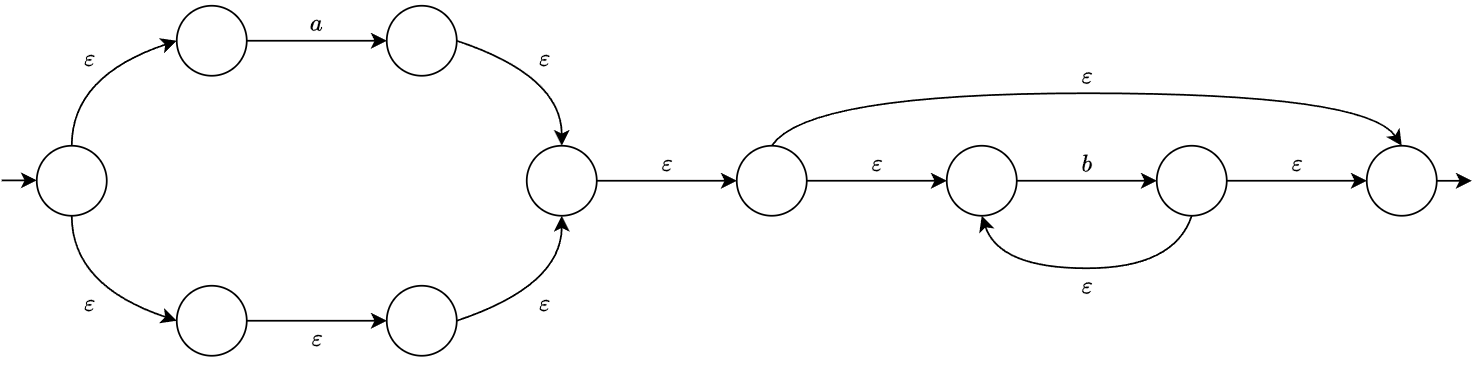
\includegraphics[width=0.75\linewidth]{images/at.png}
    \end{figure}
    The found automaton can be optimized to avoid redundant states.
\end{example}

\subsection{Glushkov McNaughton Yamada method}
The Glushkov-McNaughton-Yamada (GMY) algorithm is employed to construct an automaton equivalent to a given regular expression. 
The algorithm assigns states in a one-to-one correspondence with the generators occurring in the regular expression.
The GMY algorithm, grounded in the linearity of regular expressions, follows these steps:
\begin{enumerate}
    \item Enumerate the regular expression $e$ and derive the linear regular expression $e_{\#}$.
    \item Compute the three characteristic local sets (Ini, Fin, Dig) of $e_{\#}$.
    \item Design the recognizer for the local language generated by $e_{\#}$.
    \item Remove the indexing, resulting in the recognizer for $e$.
\end{enumerate}
\begin{example}
    Consider the regular expression $e=(ab)^{\ast}a$.
    Applying the GMY algorithm involves the following steps:
    \begin{enumerate}
        \item Enumerate the regular expression, obtaining: 
            \[e_{\#}=(a_1b_2)^{\ast}a_3\]
        \item Compute the sets:
            \begin{itemize}
                \item $\textnormal{Ini}(e)=\{a\}$.
                \item $\textnormal{Fin}(e)=\{a\}$.
                \item $\textnormal{Dig}(e)=\{ab,ba\}$.
            \end{itemize}
        \item Construct the recognizer for the numbered expression:
            \begin{figure}[H]
                \centering
                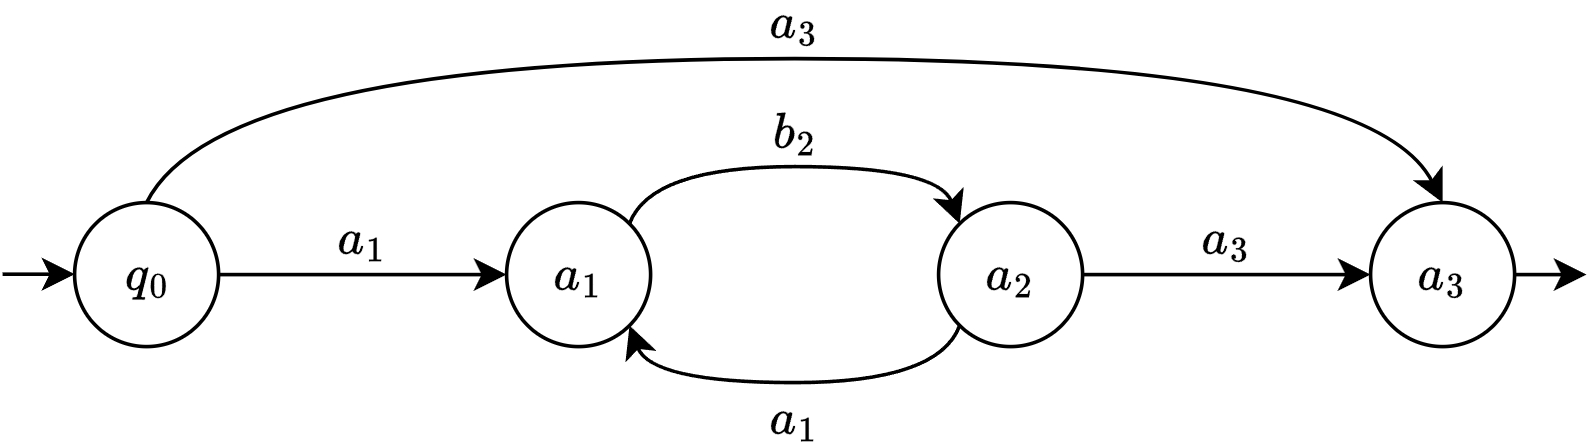
\includegraphics[width=0.75\linewidth]{images/gmy1.png}
            \end{figure}
        \item Remove the enumeration: 
            \begin{figure}[H]
                \centering
                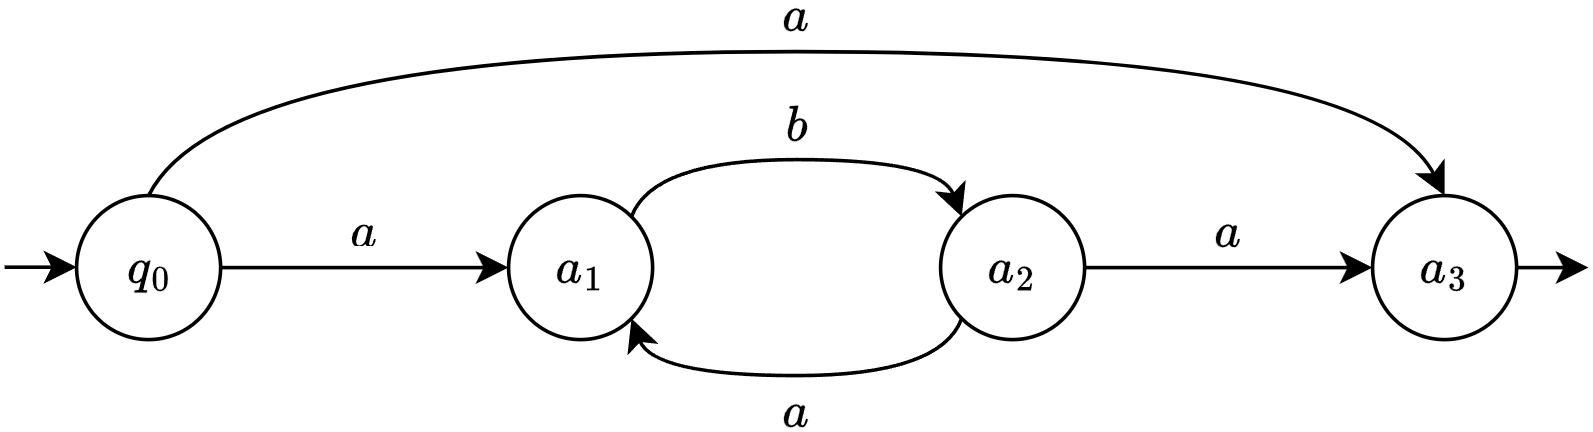
\includegraphics[width=0.75\linewidth]{images/gmy2.png}
            \end{figure}
    \end{enumerate}
    The result is a non-deterministic automaton without spontaneous moves, featuring as many states as there are occurrences of generators in the regular expression, plus one additional state.
\end{example}

\subsection{Berry-Sethi method}
To obtain the deterministic recognizer, we can apply the subset construction to the non-deterministic recognizer generated by the GMY algorithm. 
However, a more direct algorithm known as Berry-Sethi exists.
The underlying idea of the Berry-Sethi algorithm is as follows:
\begin{enumerate}
    \item Consider the end-marked regular expression $e \dashv$ instead of the original regular expression $e$.
    \item Let $e$ be a regular expression over the alphabet $\Sigma$, and let $e_{\#}$ be the numbered version of $e$ over $\Sigma_{\#}$ with the Null predicate and local sets Ini, Fin, and Dig.
    \item Define the set Fol as follows:
        \begin{enumerate}
            \item $\textnormal{Fol}(c_{\#}) \in \wp (\Sigma_{\#} \cup \{\dashv\})$. 
            \item $\textnormal{Fol}(\dashv)=\varphi$.
            \item $\textnormal{Fol}(a_i)=\{b_j\mid a_ib_j \in \textnormal{Dig}(e_{\#}\dashv)\}$ where $a_i$ and $b_j$ may coincide. 
        \end{enumerate} 
    \item Apply the subsequent algorithm.
\end{enumerate}
\begin{algorithm}[H]
    \caption{Berry-Sethi}
        \begin{algorithmic}[1]
            \State $q_0 = \text{Ini}(e_{\#} \dashv)$
            \State $Q = \{q_0\}$
            \State $\delta = \varnothing$
            \While{$\exists q \in Q\mid q$ is unmarked}
                \State Mark state $q$ as visited
                \For{$\forall c \in \Sigma$}
                    \State $q^{\prime} = \bigcup_{\forall c_{\#} \in \Sigma_{c_{\#}}}\text{Fol}(c_{\#})$
                    \If {$q^{\prime} \neq \varnothing$}
                        \If {$q^{\prime} \notin Q$}
                            \State Set $q^{\prime}$ as a new unmarked state
                            \State $Q = Q \cup \{q^{\prime}\}$
                        \EndIf
                        \State $\delta = Q \cup \{q^{\prime}\}$
                    \EndIf
                \EndFor
            \EndWhile
        \end{algorithmic}
\end{algorithm}
\begin{example}
    Apply the Berry-Sethi (BS) algorithm to the language, starting with the enumeration of the string:
    \[e_{\#}=(a_1\mid b_2b_3)^{\ast}(a_4c_5)^{+} \dashv\]
    The characteristic sets are defined as follows:
    \begin{itemize}
        \item $\textnormal{Ini}(e_{\#})=\{a_1,b_2,a_4\}$.
        \item $\textnormal{Fin}(e_{\#})=\{\dashv\}$.
        \item $\textnormal{Dig}(e_{\#})=\{a_1a_1,a_1b_2,a_1a_4,b_2b_3,b_3a_1,b_3b_2,b_3a_4,a_4c_5,c_5a_4,c_5\dashv\}$.
    \end{itemize}
    The table of followers is given by:
    \begin{table}[H]
        \centering
        \begin{tabular}{cc}
        \hline
        \textbf{$\boldsymbol{c_{\#}}$} & \textbf{Fol$(\boldsymbol{c_{\#}})$} \\ \hline
        $a_1$                          & $a_1b_2a_4$                         \\
        $b_2$                          & $b_3$                               \\
        $b_3$                          & $a_1b_2a_4$                         \\
        $a_4$                          & $c_5$                               \\
        $c_5$                          & $a_4\dashv$                         \\ \hline
        \end{tabular}
    \end{table}
    The resulting automaton is depicted in the following figure:
    \begin{figure}[H]
        \centering
        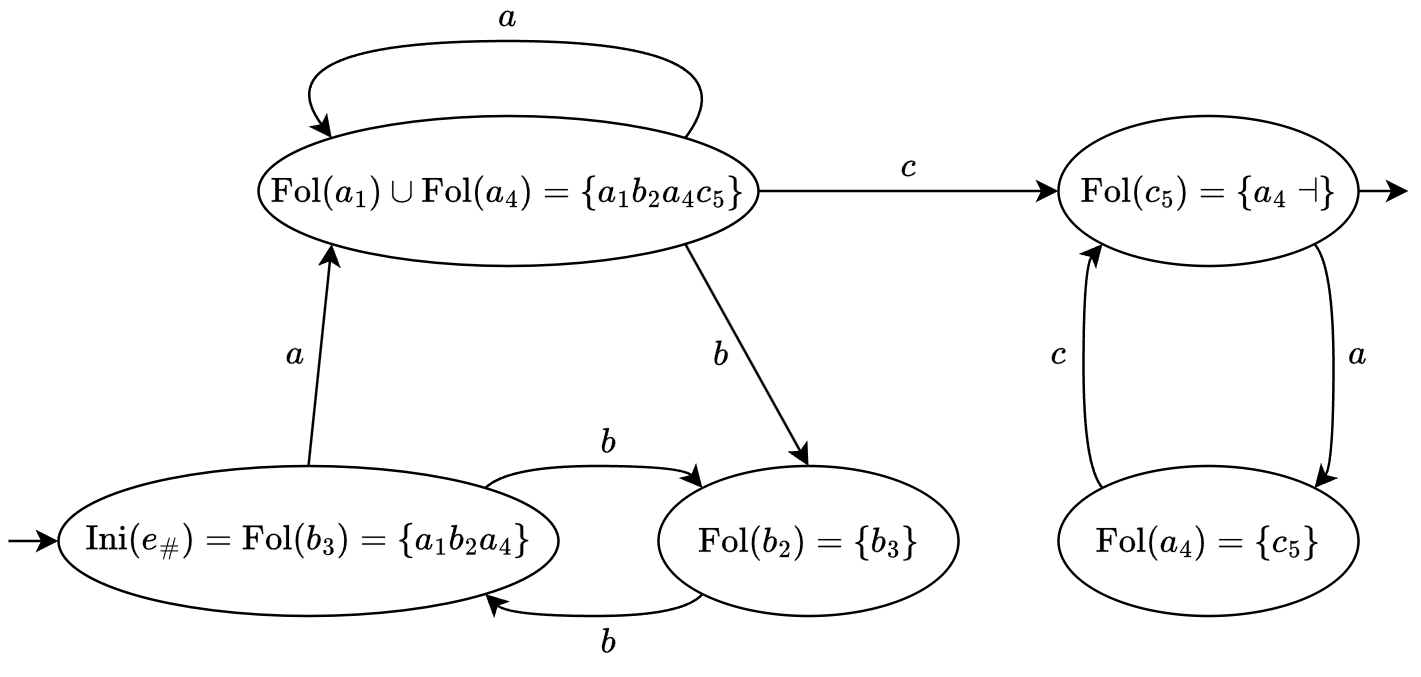
\includegraphics[width=0.7\linewidth]{images/bs.png}
    \end{figure}
\end{example}
The Berry-Sethi algorithm provides a method for converting a nondeterministic automaton into a deterministic one. 
The procedure involves the following steps:
\begin{enumerate}
    \item Enumerate the elements present on the arcs.
    \item Generate the followers table based on the enumerated elements.
    \item Reconstruct the automaton using the information from the followers table.
\end{enumerate}

\begin{example}
    Consider the given automaton:
    \begin{figure}[H]
        \centering
        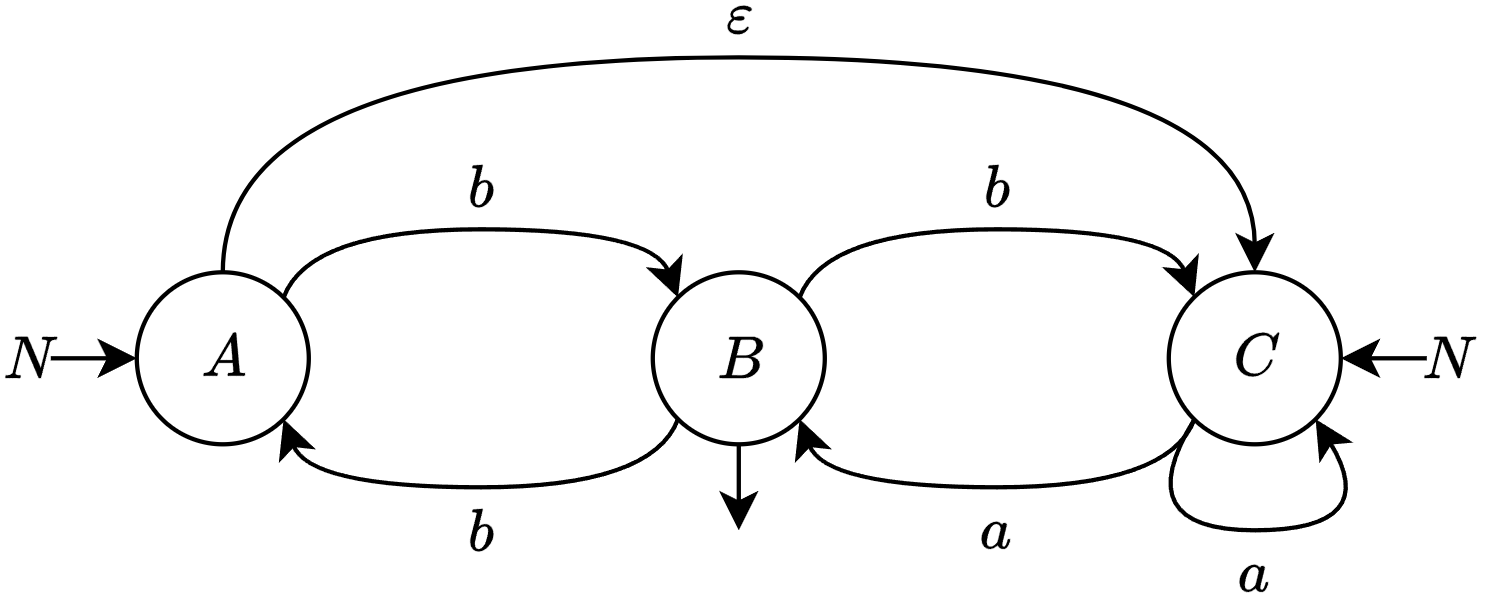
\includegraphics[width=0.5\linewidth]{images/bs1.png}
    \end{figure}
    Its numbered version is as follows:
    \begin{figure}[H]
        \centering
        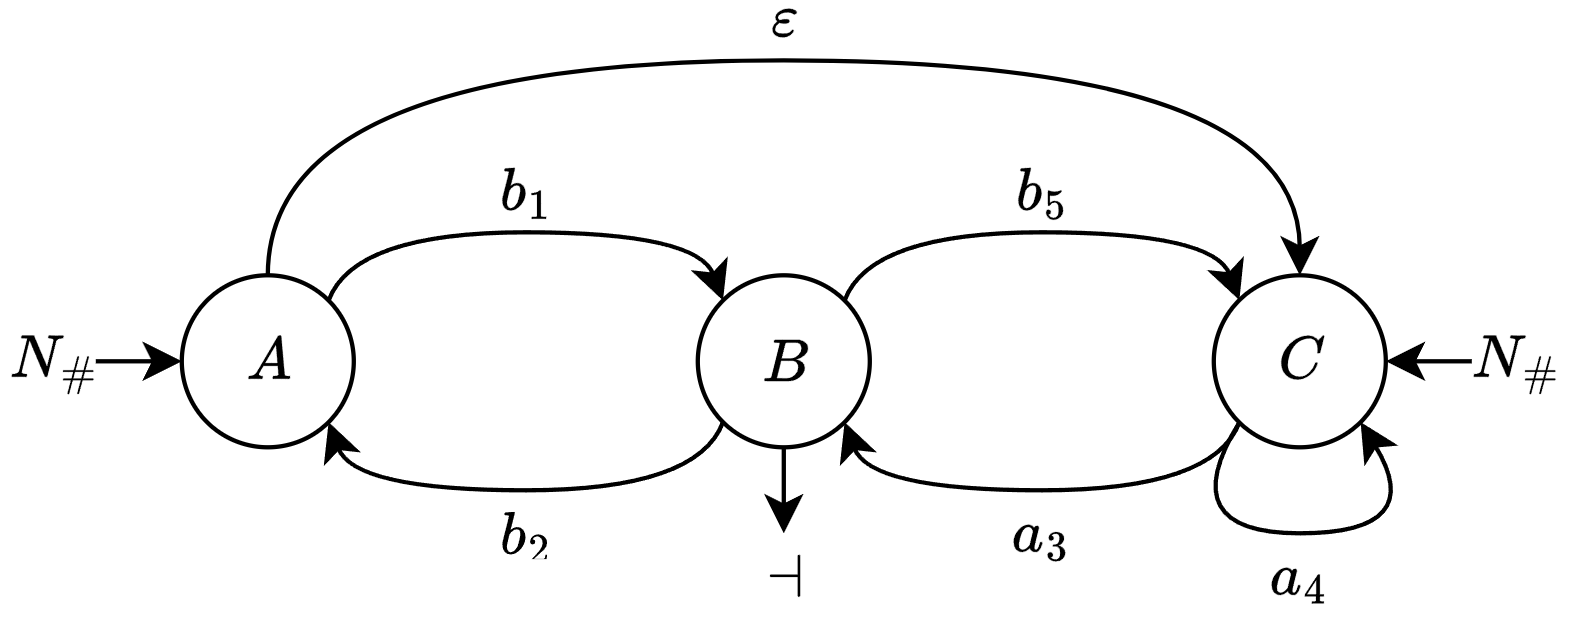
\includegraphics[width=0.5\linewidth]{images/bs2.png}
    \end{figure}
    The corresponding follower table is provided below:
    \begin{table}[H]
        \centering
        \begin{tabular}{cc}
        \hline
        \textbf{$\boldsymbol{c_{\#}}$} & \textbf{Fol$(\boldsymbol{c_{\#}})$} \\ \hline
        $b_1$                          & $b_2b_5\dashv$                      \\
        $b_2$                          & $b_1a_3a_4$                         \\
        $a_3$                          & $b_2b_5\dashv$                      \\
        $a_4$                          & $a_3a_4$                            \\
        $b_5$                          & $a_3a_4$                            \\ \hline
        \end{tabular}
    \end{table}
    The resulting deterministic automaton is depicted below:
    \begin{figure}[H]
        \centering
        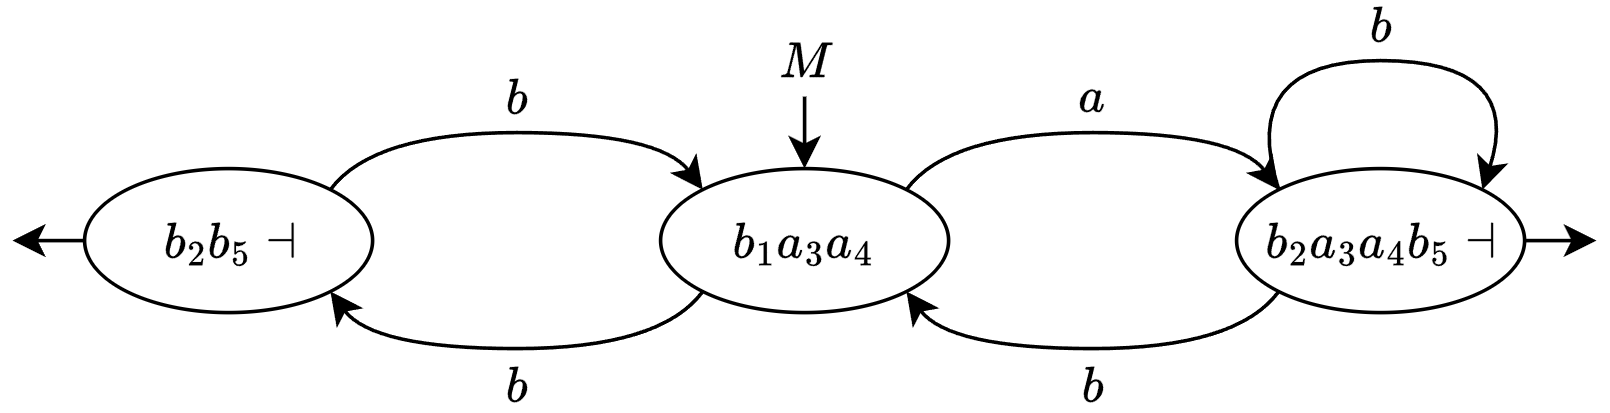
\includegraphics[width=0.7\linewidth]{images/bs3.png}
    \end{figure}
\end{example}